%-------------------------------------
\subsection{Beacons}
Los Beacons son pequeños dispositivos de posicionamiento que emiten señales Bluetooth 4.0 o BLE, mediante los cuales se puede realizar el envío de cualquier información cifrada a dispositivos que dispongan de este tipo de conectividad que se encuentren en un radio de acción de hasta 200 metros. Estos dispositivos funcionan de forma autónoma sin necesidad de carga y  pueden ser colocados en diferentes tipos de superficies dentro de establecimientos con el fin de enviar y recibir información sobre el mismo \cite{Beacon1}. 
\\ \par
En la figura \ref{imagen:arquitecturaBeaon} podemos observar los 3 elementos que constituyen internamente al Beacon, estos componentes son: la carcasa que cubre al emisor Bluetooth, dicho emisor y una pequeña pila que tendrá una duración de entre 1 y 5 años. 
\FloatBarrier
\begin{figure}[htbp!]
		\centering
			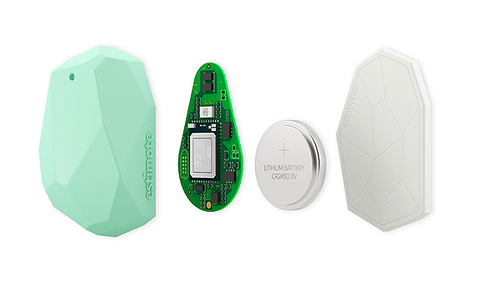
\includegraphics[width=.5 \textwidth]{imagenes/beacon_archi}
		\caption{Arquitectura interna del Beacon \cite{Beacon2}.}
		\label{imagen:arquitecturaBeaon}
\end{figure}
\FloatBarrier
\subsubsection{Firmware}
El firmware en los Beacons es específico según el proveedor de estos y este permite controlar diferentes características tales como:
\\
- Potencia de transmisión ó Tx Power, que se refiere a la potencia fija con la que los Beacons transmiten una señal, misma que disminuye a medida que se incrementa la distancia \cite{Beacon3}.\\
- Intervalo de emisión, que define la frecuencia con la que emite una señal el Beacon. Este intervalo  dependerá del tiempo de emisión ya que en cuanto más bajo sea este intervalo, más energía será consumida por el dispositivo \cite{Beacon3}. 
\\ \par
\subsubsection{Ventajas}
\FloatBarrier
\begin{itemize}
\item El tamaño de los Beacons es cómoda para las empresas, ya que va desde los 6 mm. hasta los 27 mm \cite{Ventajas}.
\item No requieren ser cargados debido a que trabajan con Bluetooth Low Energy \cite{Ventajas}.
\item Para el usuario la tecnología no resulta ser intrusiva puesto que antes de recibir notificaciones, debe instalar la app de la compañía que ofrece el servicio \cite{Ventajas}.
\item La tecnología Bluetooth no depende de ninguna red de datos, por lo cual no consume la tarifa de datos del usuario \cite{Ventajas}.
\item Permite conocer la geolocalización indoor del usuario \cite{Ventajas}. 
\end{itemize}


Se muestra a continuación la tabla comparativa \ref{Beacons} entre los distintos Beacons existentes en el mercado, en la cual se puede visualizar la que el equipo ha seleccionado para este trabajo (Estimote) y las características que tanto la elegida como las demás proveen.

\FloatBarrier
\begin{table}[htb]
\setlength\extrarowheight{2pt} % for a bit of visual "breathing space"
\begin{tabularx}{\textwidth}{|C|C|C|C|C|C|C|}
\hline
\textbf{Beacons / Características} & \textbf{Estimote} & \textbf{BlueSense} & \textbf{Gelo} & \textbf{Gimbal} & \textbf{Kontakt} & \textbf{Sonic Notify} \\\hline
Reconocimiento & Han distribuido más  de 10,000 kits. Próximos a convertirse en líderes manufactureros. Cuentan con su propia SDK & Son la empresa emergente con más reconocimiento en Reino Unido. & Funcionan en todo tipo de clima. & Desarrollados por Qualcomm, la única empresa grande de hardware que ha decidido manufacturar Beacons. & Los favoritos en Beekn, blog dedicado especialmente a Beacons. & Los favoritos en Beekn, blog dedicado especialmente a Beacons. \\ \hline
Desventajas &  Su SDK se encuentra en constantes actualizaciones. & Aún están trabajando en su SDK. & Sólo tienen soporte para iBeacon. & Se requiere pagar una fianza de utilización. & La fuerza de la señal depende de la orientación del Beacon. & Únicamente son vendidos a empresas de marketing. \\ \hline
Alcance máximo & 70 metros & 100 metros &  S/I & 50 metros &  70 metros &  S/I \\ \hline
Duración de batería & 2 años & 2 años & 2 años & 2-3 meses & 4 años & S/I \\ \hline
Precio por paquetes & \$1,133.39 por 3 Beacons. & \$1,133.39 por 3 Beacons. & \$1,325.57 por 2 Beacons. & \$77.91 por 1 Beacon. & \$1,153.6 por 3 Beacons. & \$1,153.6 por 3 Beacons. \\ \hline
\end{tabularx}
\end{table}
\FloatBarrier

\subsection{Bluetooth Low Energy (BLE)}
El BLE, es una nueva tecnología digital de radio (inalámbrica) interoperable para pequeños dispositivos desarrollada por Bluetooth. Esta tecnología y el Bluetooth 4.0 son soportados por diferentes plataformas como:
\FloatBarrier
\begin{itemize}
\item iOS5+ / iOS7
\item Android 4.3+
\item Apple OS X 10.6+
\item Windows 8
\item GNU/Linux 4.93+ \cite{Bluetooth1}
\end{itemize}

BLE hace uso del Generic Access Profile(GAP) y del Generic Attribute Profile(GATT). 
\\
El GAP es responsable de definir la topología general de la red del BLE. Esta capa realiza el manejo de los modos de acceso y procedimientos del dispositivo tales como el descubrimiento del dispositivo (permitir que sea público o no) y determina como dos dispositivos pueden interactuar entre ellos.
\\ \par
GAP define diferentes roles para los dispositivos mismos que son categorizados en periféricos y centrales.
Los periféricos son dispositivos pequeños, de baja potencia y de bajos recursos, que pueden conectarse a dispositivos centrales mucho más potentes. Un ejemplo de periférico es el Beacon; mientras que un dispositivo central corresponde normalmente a un teléfono móvil o una tableta que tienen una capacidad de proceso mucho mayor.
\\ \par
Por otra parte el GATT describe detalladamente el proceso de transferencia de los datos una vez que los dispositivos tienen una conexión establecida. Este se enfoca especialmente en como los datos son formados, empaquetados y enviados según las reglas descritas \cite{Bluetooth2}.
